\documentclass[root.tex]{subfiles}

\begin{document}
	
	{\pagestyle{empty}}
	\section{Showcase Maneuver}
	\label{chap:Showcase_Maneuver}
	To briefly show the general functioning and to give the reader insight into a practical application of the project, a standard driving maneuver was performed on the platform. As an example the U-turn was chosen, for its relevance in everyday driving and the fact that it shows some of the characteristics of \gls{HCT}-combinations distinctively. It was executed at a longitudinal speed of $2m/s$, thus resulting in a turning radius of approx. 16m. To eliminate ensure consistent behaviour over all measurements, the steering-angles of the truck were pre-programmed.
	
	\begin{figure}[!h]
		
		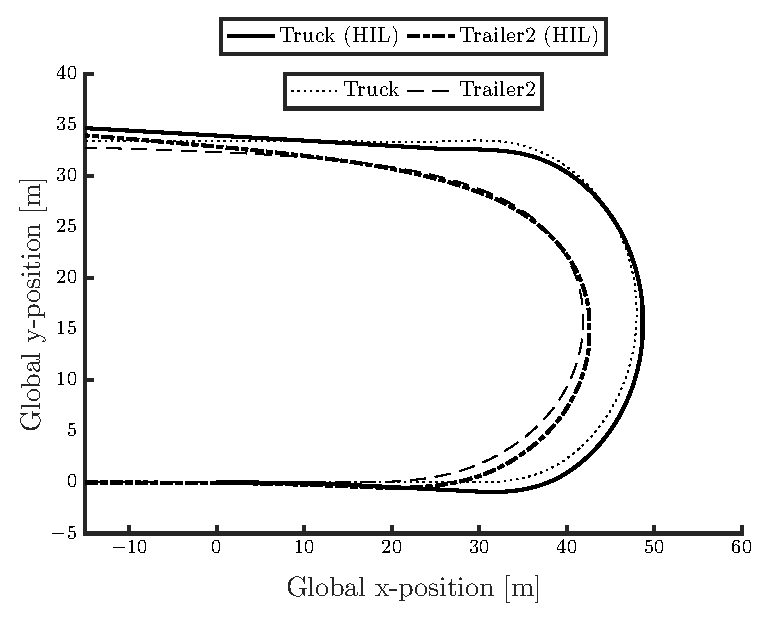
\includegraphics[width=1\linewidth]{xy_HIL_and_VTM}
		\caption[Path of Tractor and Second Trailer for HiL and Simulation]{Path of Tractor and Second Trailer for HiL and Simulation}
		
		\label{fig:Path}
	\end{figure}
	
	
	Figure \ref{fig:Path} shows the be behaviour of the different units of the combination both for the developed platform in its \gls{HIL}-configuration as well as the performance in the simulation environment. This gives the opportunity to compare between the two different stages of abstraction in the V-model, thus verifying the correct functioning of the actuated axles before executing further testing in the V-model on the test-track. 
	
	\begin{itemize}
		\item explain off-tracking as a measure 
		\item swept path deviation	
	\end{itemize}
	
\end{document}